\chapter{Agent}
In this chapter we are going to understand how the agent functions. Each agent consists from several parts which are described in detail.

\section{Agent Architecture}
Before seeing each part of the agent's software separately, it is time to describe the framework's architecture.  Soccer Simulation Server known as rcssserver3d is responsible for sending to our agent perception messages. Communication layer is the one that handles all the received messages and pass them to the agent. In agent layer, these messages are handled by a message parser which is responsible for updating all beliefs of the agent. Consequently, all functions that require new perceptions start then. Now, agent is free to do what the behavior tells him.
In our approach, only goalkeeper is running an independent behavior, the other eight field players start a communication procedure in order to inform the goalkeeper about the worldstate and their attributes. So, we can realise that field players do not execute any behavior. We are going to describe coordination procedure later in a separate chapter.
Communication controller and motion controller are responsibe for handling the agent's requests for a message that he has to say or a movement that he has to execute. These two controller are sending in every cycle effection messages to the connection layer which will send them back to soccer simulation server.\\
\begin{figure}[!h]
\centering
  \includegraphics[trim=1cm 2cm 1cm 2cm, clip=true,scale=0.7]{Chapter3/figures/Architecture.pdf}
  \caption{Agent's Architecture.}
  \label{fig:Architecture}
\end{figure}

\section{Connection}
The SimSpark server hosts the simulation process that manages the simulation. It is responsible for advancing the simulation. So, each agent
connects to this server. Agents receives messages from the server every 20ms; These messages includes information about all agent's perceptions.As we can see in the figure \ref{fig:Simulation-Update-Loop}, SimSpark Server send to agents sense messages in the beggining of every cycle. Each agent who is willing to send an action message, can send it in the end of his cycle, Server is going to receive at the same time it will send the next sense message.
\begin{figure}[!ht]
\centering
  \includegraphics[scale=0.4]{Chapter2/figures/800px-SimulationUpdateLoopSynchronizationBetweenSimSparkAndAgent.png}
  \caption{Simulation Update Loop.}
  \label{fig:Simulation-Update-Loop}
\end{figure}



\section{Perceptions}
Perceptions in simulation soccer are quite different in comparison with a real robots' competition. We do not receive data from agent's sensors but from the server, which send them to us in every cycle. These messages have this form:\\
\begin{verbatim}
(time (now 46.20))(GS (t 0.00) (pm BeforeKickOff))(GYR (n torso)
(rt 0.00 0.00 0.00))(ACC (n torso) (a 0.00 -0.00 9.81))(HJ (n hj
1)(ax 0.00))(HJ (n hj2) (ax 0.01))(See (G2R (pol 14.83 -11.81 1.
08))(G1R (pol 14.54 -3.66 1.12)) (F1R (pol 15.36 19.12 -1.91))(F
2R (pol 17.07 -31.86 -1.83)) (B (pol 4.51 -26.40 -6.15)) (P (tea
m AST_3D)(id 8)(rlowerarm (pol 0.18 -35.78 -21.65)) (llowerarm (
pol 0.19 34.94-21.49)))(L (pol 8.01 -60.03 -3.87) (pol 6.42 51.1
90 -39.13 -5.17))(L (pol 5.91 -39.06 -5.11) (pol 6.28-29.26 -4.8
8)) (L (pol 6.28 29.34 -4.95)(pol 6.16 -19.05 -5.00)))(HJ(n raj1
) (ax -0.01))(HJ (n raj2) (ax -0.00))(HJ (n raj3)(ax -0.00))(HJ(
n raj4) (ax 0.00))(HJ (n laj1) (ax 0.01))(HJ (n laj2) (ax 0.00))
\end{verbatim}
The above message is just an example message our agent has been sent 
during game time. It includes information about the server time, the game state and time, the values of each one of his joints and data from vision, acceleration, gyroscope and force sensors.
\begin{figure}[!ht]
\centering
  \includegraphics[scale=0.4]{Chapter3/figures/MessagesBeliefs.jpg}
  \caption{Beliefs Update.} 
  \label{fig:BeliefsUpdate}
\end{figure}
\\




\section{Localization}
Once we have all the neccessary beliefs updated, it is time for us to use them in order to locate our agent in the field. Localization is created by Vassilis Papadimitriou in winter's 2011-2012 class Autonomous Agents. A brief description of the localization process is following.\\
\\
{\bf Localization Process}\\
\\
Localization process is executed every three cycles and when we receive observations from the vision perceptor. If we have visible objects in our sight we organize them in terms of their type. There are three types: Landmarks, Co-Players and Opponent Players. We make use of the Landmarks to find our position in the field.
The Nao's restricted vision perceptor limits the field of view to 120 degrees.
\begin{figure}[!ht]
\centering
  \includegraphics[scale=0.3]{Chapter3/figures/Localization1.png}
  \caption{Nao's field of view.} 
  \label{fig:fieldofview}
\end{figure}
An example of this limitation is described in the figure \ref{fig:fieldofview}.
Localization process became possible through three main functions. The first function, takes two landmarks as arguments and returns to us a possible position for our agent. If our agent sees more than two landmarks, then this function is called for every combination of two landmarks and in the end we calculate the average position. If our agent sees less than two landmarks, then he has a complete unawareness of his position in the soccer field. The figure \ref{fig:Localization} shows how this function works.
\begin{figure}[!ht]
\centering
  \includegraphics[scale=0.3]{Chapter3/figures/Localization3.png}
  \caption{Localization.} 
  \label{fig:Localization}
\end{figure}
Except from the calculation of our position in the soccer field, localization is responsible to locate ball and other agents in the field. Knowing our position helps us locate other objects too. For every other object which is locates in our field of view, vision perceptor informs us about its vertical angle, its horizontal angle and its distance from our agent. This information is enough for the calculation of their exact positions. Finally, after the localization process end, we are able to have the following observations:\\
\begin{description}
	\item[Our Position] Only if our agent sees more than one landmarks.
	\item[Body Angle] Only if our agent knows his position.
	\item[Other Agents Positions]	Only if our agent knows his position and other agents are located in the field of his view.
	\item[Ball Position] Only if our agent knows his position and ball is located in the field of his view.
\end{description}
In the following figure \ref{fig:LocalizationResults} we can see the results which are given by the localization process.
\begin{figure}[!ht]
\centering
  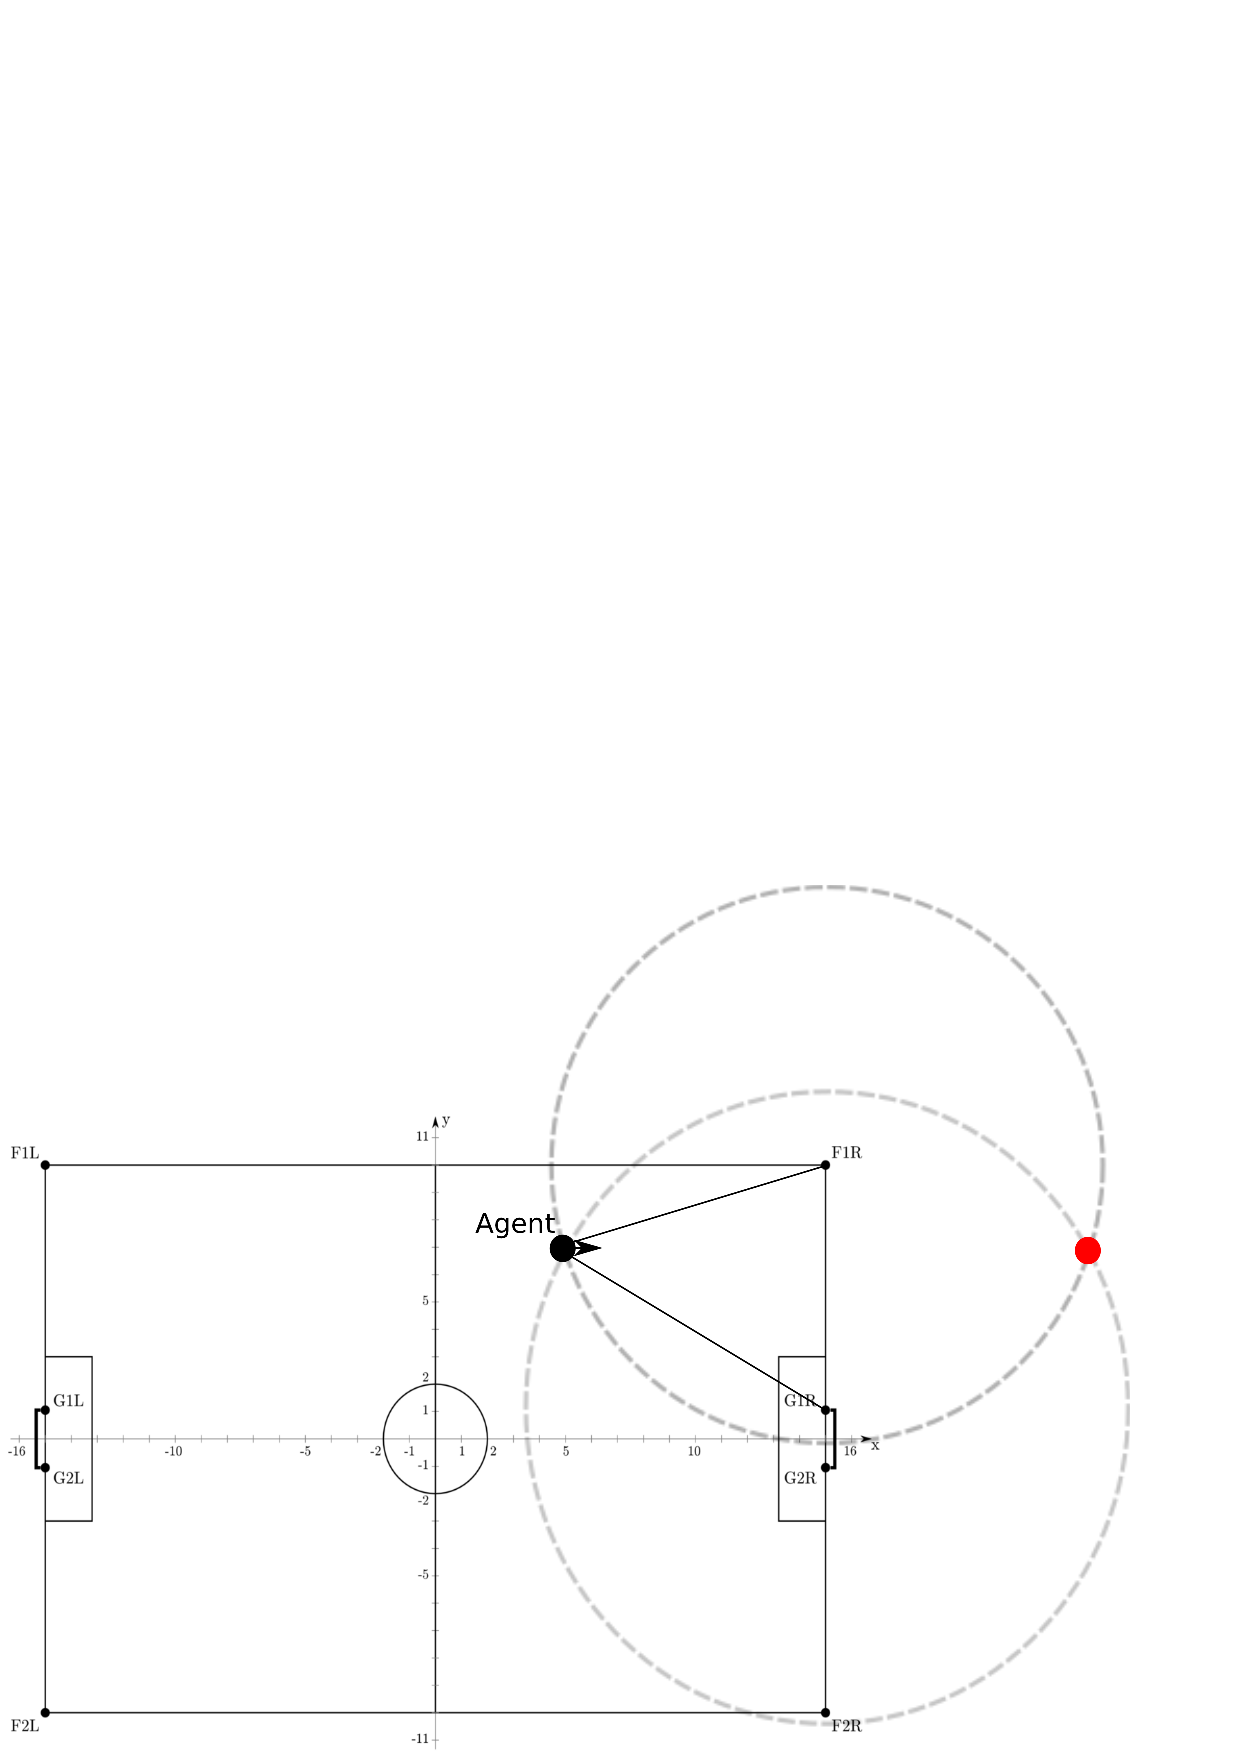
\includegraphics[scale=0.3]{Chapter3/figures/Localization.png}
  \caption{Localization Results.} 
  \label{fig:LocalizationResults}
\end{figure}


\section{Localization Filtering}
In absence of a stochastic localization, we are forced to ensure that localization results are good enough for us to rely on.Due to the symmetry of the field's landmarks, localization is not always accurate enough to depend on. This, requires a kind of filtering for the observations we take by the localization process.
\begin{algorithm}[h!]
\caption{Localization Filtering$(Observation(x,y))$}
\label{alg1}
\begin{algorithmic}[1]
\IF{$x,y \neq NaN$}
\IF{$size(Queue) = 0$}
\STATE $Queue.Add(Observation)$
\ELSIF{$size(Queue) < Max$}
\IF{$Observation \not\approx AVG(Queue)$}
\STATE $Queue.Remove()$
\ELSE
\STATE $Queue.Add(Observation)$
\STATE $MyPosition = AVG(Queue)$
\ENDIF
\ELSE
\IF{$Observation \not\approx AVG(Queue)$}
\STATE $Queue.Remove()$
\ELSE
\STATE $Queue.Remove()$
\STATE $Queue.Add(Observation)$
\STATE $MyPosition = AVG(Queue)$
\ENDIF
\ENDIF
\ENDIF
\end{algorithmic}
\end{algorithm}
The above algorithm \ref{alg1} describes the process of localization filtering. The general idea that we follow in our approach is that if our agent takes one thousand observations per minute it will be easy for him to not to take into consideration the observations with the biggest fault. In general, localization provides us with not consecutive faulty observations. To overcome this difficulty, we came up with a simple and clever approach. A queue full of observations is always gives us our agent's position in the field. When an observation is coming, we check if the queue is empty or full; If it is emtpy then we just add the observation into the queue. If it is full of elements, then we check if the new observation seems faulty in comparison to the average of the queue. If it seems faulty, we do not take it into account and we just remove an element from the queue. If not, then we add it to the queue.
If queue is neither empty nor full, then we make the same procedure checking if it is a faulty observation, with the only difference that we do not remove any element if it is not.Localization filtering applies for both the calculation of our agent's position and the ball's position. Its result was the improvement of the localization results in an adequate degree in order to rely on them with more confidence. This filtering smooths the belief of our position and rejects every faulty observation.







\section{Motions}
In robotics, we could define a motion as a sequence of joint poses. A pose is a set of values for every joint in the robot's body at a given time.
For example, for a given set of n-joints a pose could be defined as:\\
\begin{center}
$Pose(t)$=$\lbrace J_{1}(t),J_{2}(t),...,J_{n}(t) \rbrace$\\
\end{center}
Motions are very important part of every team take part in the simulation league. Most of the teams in this league make use of dynamic movement which is a major advantage for their side. In this approach, we are using motion files. Motion files are set of poses which has static and standard values for each joint for every movement. The difference between static motion files and dynamic movement is that dunamic movement takes into consideration the center of the body's mass and the direction in which we are want to head. This movement gives to the robot better body balance and fast movement especially in situations that the robot wants to change direction or to make a turn. In this approach we are using two kinds of static motion files. Text based and Xml based motion files. Agent before initializes himself in the field read these files and saves them into the dynamic memory to be ready to use them without any need of reading them every time he needs them.



\subsection{XML Based Motions}
This motion files has been created from FIIT RoboCup 3D project. They are in xml structure and it was easy to implement them into our project. The following lines show the structure of these xml motion files.
\begin{verbatim}

		<phase name="Start" next="Phase1">
			<effectors>
				Joint Values
			</effectors>
			<duration>duration</duration>
		</phase>
		<phase name="Phase1" next="Phase2">
			<effectors>
				Joint Values
			</effectors>
			<duration>duration</duration>
		</phase>
		<phase name="Phase2"next="Phase1">
			<effectors>
				Joint Values
			</effectors>
			<duration>duration</duration>
			<finalize>Final</finalize>
		</phase>
		<phase name="Final">
			<effectors>
				Joint Values
			</effectors>
			<duration>duration</duration>
		</phase>

\end{verbatim}
It is easy to understand that each movement is splitted into phases. Each phase has a duration and values for every joint of the robot. Moreover,
every phase has an index which points to the next phase. For example, we see that the first phase ''Start'' has an index for the next phase ''Phase1''. Phases with a finalize field help us to end each movement. For example, the phase:''Phase2'' has a finalize index which points to the phase:''Final'', this means that, if we want to end this motion, we should continue the motion with the finalize phase not with the next.
\subsection{XML Based Motion Controller}
Motion controller is responsible for handling the movement requests by the agent. Agent has not access in motion controller itself but he has access in the motion trigger. We can imagine this trigger as a variable which can only be changed by the agent. Each agent declares the movement he is willing to do in this variable.
Motion controller reads this variable in every cycle and generates a string which is the result of his process.
\begin{figure}[!ht]
\centering
  \includegraphics[scale=0.4]{Chapter3/figures/motions.jpg}
  \caption{Motion Controller.}
  \label{fig:MotionController}
\end{figure}
In the figure \ref{fig:MotionController} we show the general architecture of the motion controller. Motion cotroller checks if there is a motion which is playing already. If yes, motion controller tries to finalize the playing movement in order to start playing the new requested movement.
\begin{figure}[!ht]
\centering
  \includegraphics[trim=0cm 13cm 12cm 0cm, clip=true,scale=0.7]{Chapter3/figures/XMLMotions.pdf}
  \caption{Phase Sequence.}
  \label{fig:PhaseSequence}
\end{figure}
In the next figure \ref{fig:PhaseSequence} is described the exact motion sequence. In general, Xml motions is created to include cycles. For example, walking motion has three main phases which create a cycle. If motion trigger does not change at the last phase, we will continue with the first phase not with the final. As we saw in the structure of every Xml based motion file, each phase has a set of joint values. These values is in degrees. To generate motion for our agent we need to create a motion string. This string holds info about the velocity we want to give in every joint involved in the motion phase. This velocity can be calculated by:
\\
\\
$Desired Velocity$ = $Already Joint Value$ - $Desired Joint Value$\\
\\
This is the velocity of every joint. Furthermore, every phase has a duration in which has to be executed. So, phase duration has to be divide with the duration of every server cycle. This will give us the number of cycles this phase will be playing.\\
\\
$Cycles Number = \frac {Phase Duration} {Cycle Duration}$\\
\\
Now, we have the phase's velocity and the duration in cycles. We can calculate, how much will be the speed of every joint in order to reach to the desired joint value in this time limit.\\
\\
$Velocity = \frac {Desired Velocity} {Cycles Number} degrees/cycle$\\
\\
This velocity is calculated for every joint invloved in the motion. The final output of the motion controller will be send to the server.



\subsection{Text Based Motions}
The other kind of motion files that we use is created by Webots simulator. These text based motion files have simplier structure than the Xml have. At the second row, there are the definition for all joints which are related to  each motion. For example, walking motion requires only the joints from both robot's legs. The next rows from left to right have information for the duration of each pose, the pose name and finally the joints' values for each joint in the same order as they are defined in the second row.
\begin{verbatim}
#WEBOTS_MOTION,V1.0
LHipYawPitch,LHipRoll,LHipPitch,LKneePitch,LAnklePitch,...
00:00:000,Pose1,0,-0.012,-0.525,1.05,-0.525,0.012,0,...
00:00:040,Pose2,0,-0.011,-0.525,1.05,-0.525,0.011,0,...
00:00:080,Pose3,0,-0.009,-0.525,1.05,-0.525,0.009,0,...
00:00:120,Pose4,0,-0.007,-0.525,1.05,-0.525,0.007,0,...
00:00:160,Pose5,0,-0.004,-0.525,1.05,-0.525,0.004,0,...
00:00:200,Pose6,0,0.001,-0.525,1.051,-0.525,-0.001,0,...
00:00:240,Pose7,0,0.006,-0.525,1.05,-0.525,-0.006,0,...
00:00:280,Pose8,0,0.012,-0.525,1.05,-0.525,-0.012,0,...
00:00:320,Pose9,0,0.024,-0.525,1.05,-0.525,-0.024,0,...
\end{verbatim}
\subsection{Text Based Motion Controller}
Motion controller for text based motions is based on the same principle as the Xml controller. The joint values in the motion files represent
radians. So we convert these values into degrees and then we proceed with next steps. Each pose lasts for one or two cycles depending on the speed we want each motion to be executed. This motion controller could be customized easily to perform motions differently. There are parameters that can be changed such as:
\begin{description}
	\item[Speed] How fast we want pose to be executed.
	\item[Duration]	How many cycles from pose to pose.
	\item[Pose Offset] Pose Offset = 2, we execute pose1,pose3,pose5,...
	\item[Hardness Factor]	Hardness Factor = 0.9, we multiply the velocity with this factor.
\end{description}
The velocity of every joint is calculated by:\\
\\
$Desired Velocity$ = $Already Joint Value$ - $RadiansToDegrees(Desired Joint Value)$
\\
\\
$Velocity = \frac {Desired Velocity \ast Hardness Factor} {Speed} degrees/cycle$\\
\\
This velocity is calculated for every joint invloved in the motion. The final output of the motion controller will be send to the server.





\section{Actions}
advantage





\subsection{Simple}
advantage





\subsection{Complex}
advantage





\subsection{Vision}
advantage





\section{Communication}
advantage